This module deals with the main process behind STORM, it is the shuffling algorithm.
\begin{figure}[H]
	\centering
	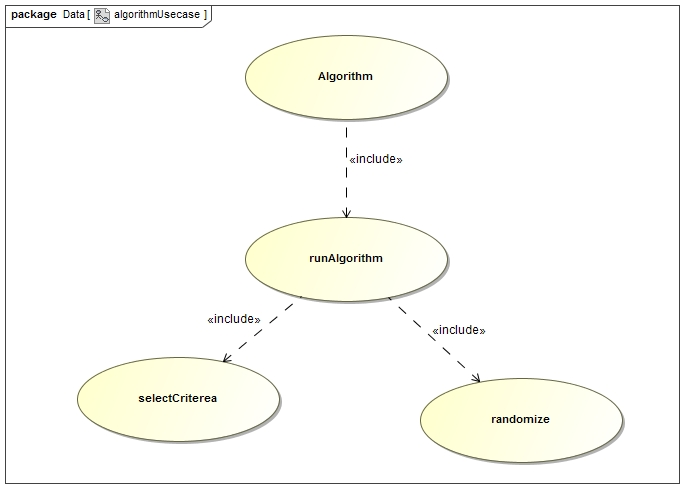
\includegraphics[width=15cm]{./graphics/algorithmUsecase.jpg}
	\caption{Algorithm module use case}
\end{figure}
\subsubsection{Use-cases}

The algorithm module adds the functionality required to shuffle subjects into teams.\par

\begin{enumerate}
\item RandomShuffle\par
Priority: Critical.\par
Pre-condition: Project must have users.\par
Pre-condition: Team size or number of teams must be specified.\par
Post-condition: Random teams are built.\par
    \begin{figure}[H]
        \centering
        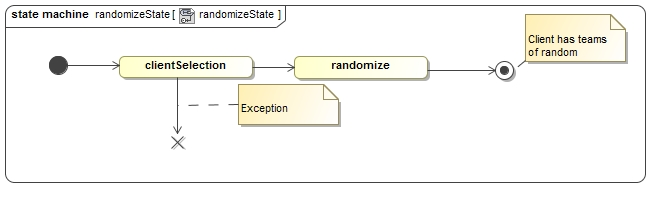
\includegraphics[width=15cm]{./graphics/randomizeState.jpg}
        \caption{Randomize state diagram}
    \end{figure}

\item SimilarShuffle\par
Priority: Critical.\par
Pre-condition: Project must have users.\par
Pre-condition: Team size or number of teams must be specified.\par
Pre-condition: Criteria with weights should be selected.\par
Pre-condition: Similar shuffle should be specified.\par
Post-condition: Similar teams are built.\par

\item DiverseShuffle\par
Priority: Critical.\par
Pre-condition: Project must have users.\par
Pre-condition: Team size or number of teams must be specified.\par
Pre-condition: Criteria with weights should be selected.\par
Pre-condition: Diverse shuffle should be specified.\par
Post-condition: Diverse teams are built.\par

\end{enumerate}
%To be completed in future iterations
\pagebreak